\section{Research Questions and Hypothesis}
    
  {\bf $H_{0}$: Human properties have no influence in users choice of graphical passwords} 

  {\bf $H_{1}$: Users choice of graphical passwords are influenced by the human properties of the user}

  The $H_{1}$ is the hypothesis I want to prove in my thesis the following sping. If the results from the analysis is proven $H_{1}$ to be correct, there can only be proven for the human properties selected in the analysis. The hypothesis do not prove that all human properties influence users choice of graphical password, but the goal for this research is not to prove all human properties. In the design of research strategy there will be a analysis of the human properties that this study find relevant to users choice in graphical patterns. 

\section{Research Strategy}

  \subsection{Selection of Research Strategy and Data Collection}

    In this thesis, the selected research strategy is a survey. To be able to answer the hypothesis there is a need for obtain data from a large group of people in a standardized and systematic way. This will provide a wide and inclusive coverage of people so the results from the data collection are likely to be representative for a wider population. 

    When selecting survey as a research strategy, a questionnaire would be a good fit for a quantitative data collection. The data properties that is selected are indicating that data needs to be collected ``world wide'', and cannot be collected face-to-face due to the lack of time and resources. For analyzing patterns in the data, a big amount of data needs to be collected. The questionnaire will be distributed over the Internet and will be helpful in the data collection process to get a sampling size that is large enough. Data collection with pen and paper are too time consuming and would not be manageable with the time available for data collection and analysis in the spring. When analyzing data, it is also necessary to have the data in a standardized format. A questionnaire is supporting a standardized format, and with a online tool it will be easy to extract the data in a standardized format for the analysis. This will provide the possibility to use automatically analysis tools without to much use of time with manually work.

    A limitations of the chosen approach is that it does not support control of the participants because the questionnaire is distributed over web, and users are not handpicked. Since the data collection is distributed over web, there is not possibility for me to judge the accuracy and honesty of peoples responses. Despite the limitations, this is chosen due to the amount of data needed for the analysis, as well as the lack of time for choosing other approaches like interviews and other observation techniques. 

    The detailed design of the questionnaire will be described in section 4.3.

  \subsection{Data Requirements}
  
  It is important to analyze what kind of human properties that may impact users choice of graphical passwords on mobile devices. We must carefully consider which human properties we want to collect in order to get a concise collection of data that can be analyzed, and further give us answer to our hypothesis. This analysis will be a review of human properties that this study find relevant to the hypothesis. As a result of this analysis, a narrowed selection of the listed human properties will further be included in the analysis.  

  \begin{itemize}
    \item {\bf Age:} A group of people within a certain group of age may have different risk awareness. A person with a age between 30-40 and a person with a age below 20 may have different concerns with security. A person in the age between 30-40 may use their phone to perform task with a high security risks like making and job related tasks, while a person with a age below 20 may not have the same security awareness because of the different use of mobile devices.
    \item {\bf Gender:} Psychological studies have reported that males are more likely to take risks than females \cite{Byrnes}. When looking at peoples choice in patterns can probability be analyzed based on gender. In the literature review there was no reported results found on genders risk awareness in information security, nor peoples choice of patterns based on gender. By analyzing peoples choice of patterns based on users gender might give interesting results. 
    \item {\bf Nationality:} This demographic information is somethimes used in research for graphical passwords. When asking a person about their PIN code, a nationality can be used to find likeley numbers to appear because som cultures associates a number to a historical or religious event. In a reseach on the passface, this property was used and proven to be valuable because people tended to choose faces from the same race and nationality. In my reseach it is uncertian how much this information will help to prove any connection to the choice of patterns. Properties like language perferance and reading/writing orientation look more promising in this reasearch.
    \item {\bf Language preference:} By asking the respondent for information about the language perferance it can be used to confirm the way a person read/write.
    \item{\bf Occupation:} This information is valuable information due to the knowlegde level of the respondents. The occupation of the a presondant are simply if the person is a student, employed, not currently employeed or retired.
    \item {\bf Profession:} The profession of a person may say something about a persons knowledge and background. When looking at profession, a person with a profession in IT may be more certain about the security aspects than people in other professions. 
    \item {\bf Left- or right handed:} An interesting property of humans is the fact that people write with either left or right hand (and sometimes both). This property can influence the way a person are holding the phone and may impact the way that a person is making a pattern. In the literature review it was not found any studies that reported any results of people choices in patterns based on the hand used. Published research \cite{Uellenbeck} found that over 40\% of interest in a study started their Android pattern by starting in the top left corner, but did not record the hand used when making the pattern. My hypothesis is that a left handed person may be using the left hand while interacting with the phone, making the probability for starting in the right upper corner bigger. This have never been tested before and need further research before making a statement. 
    \item {\bf Reading/writing orientation:} In different cultures, there is a difference in the reading and writing direction. Cultures from Europe and America is normally writing and reading horizontally from left to right, but there are other cultures that do otherwise. Traditionally, Chinese, Japanese, and Korean are writing text vertically in columns from top to bottom, from right to left. Another writing orientation is horizontal from right to left that are used in Arabic cultures. Today, the vertical orientation from top to bottom is often in a horizontal way due to the influence of English and the increased computerized typesetting, but both ways are still in use. There are research that have reported that the writing orientation are affecting the visual attention and memory \cite{Chan}. They found that the reading orientation affected the way a person would memorize objects. They reported that English and Chinese speakers tended to remember an image that appeared in the top, left-hand side of the screen and the Taiwanese speakers tended to remember the images in the upper right-hand side of the screen. The interesting aspect of this reading and writing orientation is to see if people from different cultures are choosing different patterns due to their writing orientation.
    \item {\bf Hand size:} Smartphones today tends to get bigger and bigger in size. An interesting analysis could be done by looking at a users choice of patterns based on size of their hands and size of mobile phone where a patterns is made. By looking at a situation were a person with a small hand and a big mobile device, it may be hard to reach certain areas on the screen by holding a device in one hand, and therefore impact the choice of pattern. 
  \end{itemize}

  \begin{figure}[H]
    \centering
    \subfigure{
      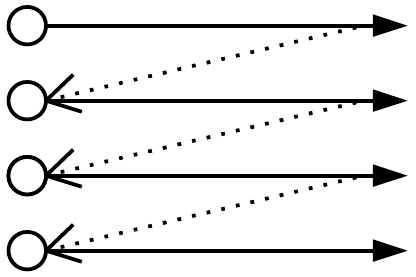
\includegraphics[scale=0.25]{pics/leftright.png}
    }
    \subfigure{
      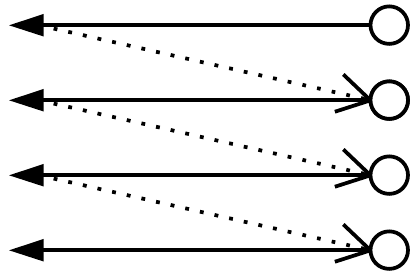
\includegraphics[scale=0.25]{pics/rightleft.png}
    }
    \subfigure{
      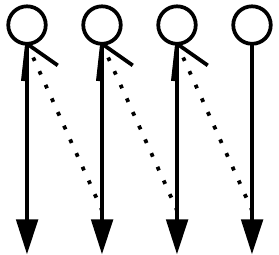
\includegraphics[scale=0.27]{pics/topbottom.png}
    }
    \caption{Writing orientatio: 1) Horizontally Left-to right, 2) Horizontally Right-to-left 3) Vertically Right-to-left}
  \end{figure}

  As a result from the analysis of different human properties above I need to make a selection that looks promising to give any results in the analysis. As stated earlier, the goal of this reseach is not to prove that all human properties will impact users choice of patters, but make a selection of human properties that I find promising to look further into. The human properties that will be included in the analysis is the  "reading/writing orientation", "hand size", "Left- or right-handed". 
  Beside the the three main selected properties, I want to collect some demographics and some background information about the users. This will further be described in section 4.3.

  \subsection{Sampling Frame and Technique}

    \todo{Er det her jeg skal nevne hvem jeg ønsker å samle inn svar fra (sampling frame)?}
    
    The survey type is categorized as ``non-probability sampling'' and the chosen sample technique is ``self-selection strategy''. This is chosen due to time and cost estimates, and the lack of control of participants. A Purposive sampling technique would maybe provide a more uniformly collection of people, but it is hard to control the participants when the questionnaire is distributed on the web. The self-selection strategy will collect data from any respondents, and will be helpful when there is big population with potential respondents. The self-selection is a useful technique when we are not able to directly contact the potential respondents. When people select themselves for research, it might indicate that they have a strong feeling on the subject, or because they think it will bring them personal benefit or approval. 

  \subsection{Response Rate and Non-responses}

    When sending out the questionnaire I have no control over how many people will participate because of the distribution of the questionnaire over the Internet. To be able to reach the amount of data need I need to look for a strategy that may increase the number of responses. If I suspect that certain types of people in my sample will be less willing to respond, I could deliberately include more of that type in my sample so I can assure that I receive the number of respondents that I need. Maybe go face-to-face if a special group of people may be less willing to participate. 

    In this table there will be described different subgroups of people that I want to get data from, but may be hard to reach with respect of different factors. There will be description of a strategy for reaching the subgroups that I predict to have less responses from:

    \begin{tabular}{| p{4cm} | p{7cm} |}
      \hline
      {\bf Subgroup} & {\bf Sampling strategy} \\ \hline
      {\bf People with age of 50 or higher} & People with the age over 50 may not own their own smaprtphone, or may be hard to reach for other reasons. I need to find networks were there is a high representation of people with a age over 50. In Norway there is a network ``Seniorweb'' and a magazine called ``vi over 60'' that is a network that is highly represented with people with an age over 50. \\ \hline
      {\bf People with a different field of interest than IT} & My own network is overepresented by people with a profession in IT and security. I need to be able to find other networks to be able to reach out to other people wither other professions. \\ \hline
      {\bf People with a reading orientation from right-to-left} & The main reading orientation is from right-to-left, with a exception with some arabic an asian natinalities. \\ \hline
      {\bf People living in a different country than Norway} & I need to get in touch with persons from different nationalities to get diversity in the data. I will contact the International Section at my university to ask them to distribute my questionnaire to the exchange students at my university. I am also having a trip to Minnesota in USA in the following spring, and I will use my time there recruiting people to respond to my questionnaire. During this semester I have been talking to researchers in other countries because of their interest in my research. Hopefully I can get help to distribute the questionnaire within their network. \\ \hline
      {\bf People that are left-handed} & There is a significant higher percentage of people that are right-handed, meaning that there is a possibility for recruiting more people that are right-handed. Selecting a strategy for this is hard because there is no forum for left-handed people. If there are few respondents that are left-handed I need to directly look for people that are left-handed at my school.\\ \hline
    \end{tabular}

    When analyzing the collected data in the following spring, I need to find characteristics of people that have not answered to make a discussion of why they didn't (maybe they are not representative), or whether their non-response is meaningful in its own right, or whether their lack of responses has resulted bias in my final sample. This part is out of scope for this thesis, but need to be considered in my thesis next semester.
  
  \subsection{Sample Size}
    I need to decide how big I want my final sample to be, taking into account my best estimate of the likely non-response rate of participants. When looking at my target population that is a very wide range. My target population is higher than 1 million, and therefore I would probably need 1000 respondents or more..

    Because of the lack of control of the diversity of the respondants, there is likely to be some data properties that have a higher representation that others. Therefore it is important to control the data collected during the sping. If it I get a situation where a subpopulation is overrepresented, it is desired to have a strategy for smoothing the data. The data collected should never be manipulated, and in a situation where there is lack of respondents from a subgroup the only thing that I can do is to contact networks were the missing population have a higher possibility to be reached. A strategy is described in section 4.2.4. 

    The total sample size is quite high, but should be manageable. If the total amount of 1000 respondents is not reached, a minimum number of respondents should be accepted at 500. In the analysis it will be hard to make any conclusions if the total number of respondants is too low.  The Internet offers researchers the possibility of accessing many people across the world cheaply and quickly. Not everyone have Internet access, and that need to be considered in the design. Maybe they are not a targeted group since this is a mobile focus.

